% !TeX root = ../../main.tex
\section{Breakdown of capital costs} \label{app:capexbreakdown}
\begin{table}[H]
\centering
\caption{Installation factors for factorial estimate method}
\label{tab:Installation factors}
\begin{tabular}{lll}
\toprule
\textbf{Item}                & \textbf{Value} & \textbf{Description}                                        \\\midrule
$f_{er}$                       & 0.5            & Installation factor for equiment erection                   \\
$f_{p}$                        & 0.6            & Installation factor for piping                              \\
$f_{i}$                        & 0.3            & Installation factor for instrumentation and process control \\
$f_{el}$                       & 0.2            & Installation factor for electrical work                     \\
$f_{c}$                        & 0.3            & Installation factor for civil engineering work              \\
$f_{s}$                        & 0.2            & Installation factor for structures and buildings            \\
$f_{l}$                        & 0.1            & Installation factor for lagging, insulation or paint        \\
$f_{m}$                        & 1.3            & Material cost factor                                        \\
\textbf{Installation factor} & \textbf{3.68}  &                                                            \\\bottomrule
\end{tabular}
\end{table}

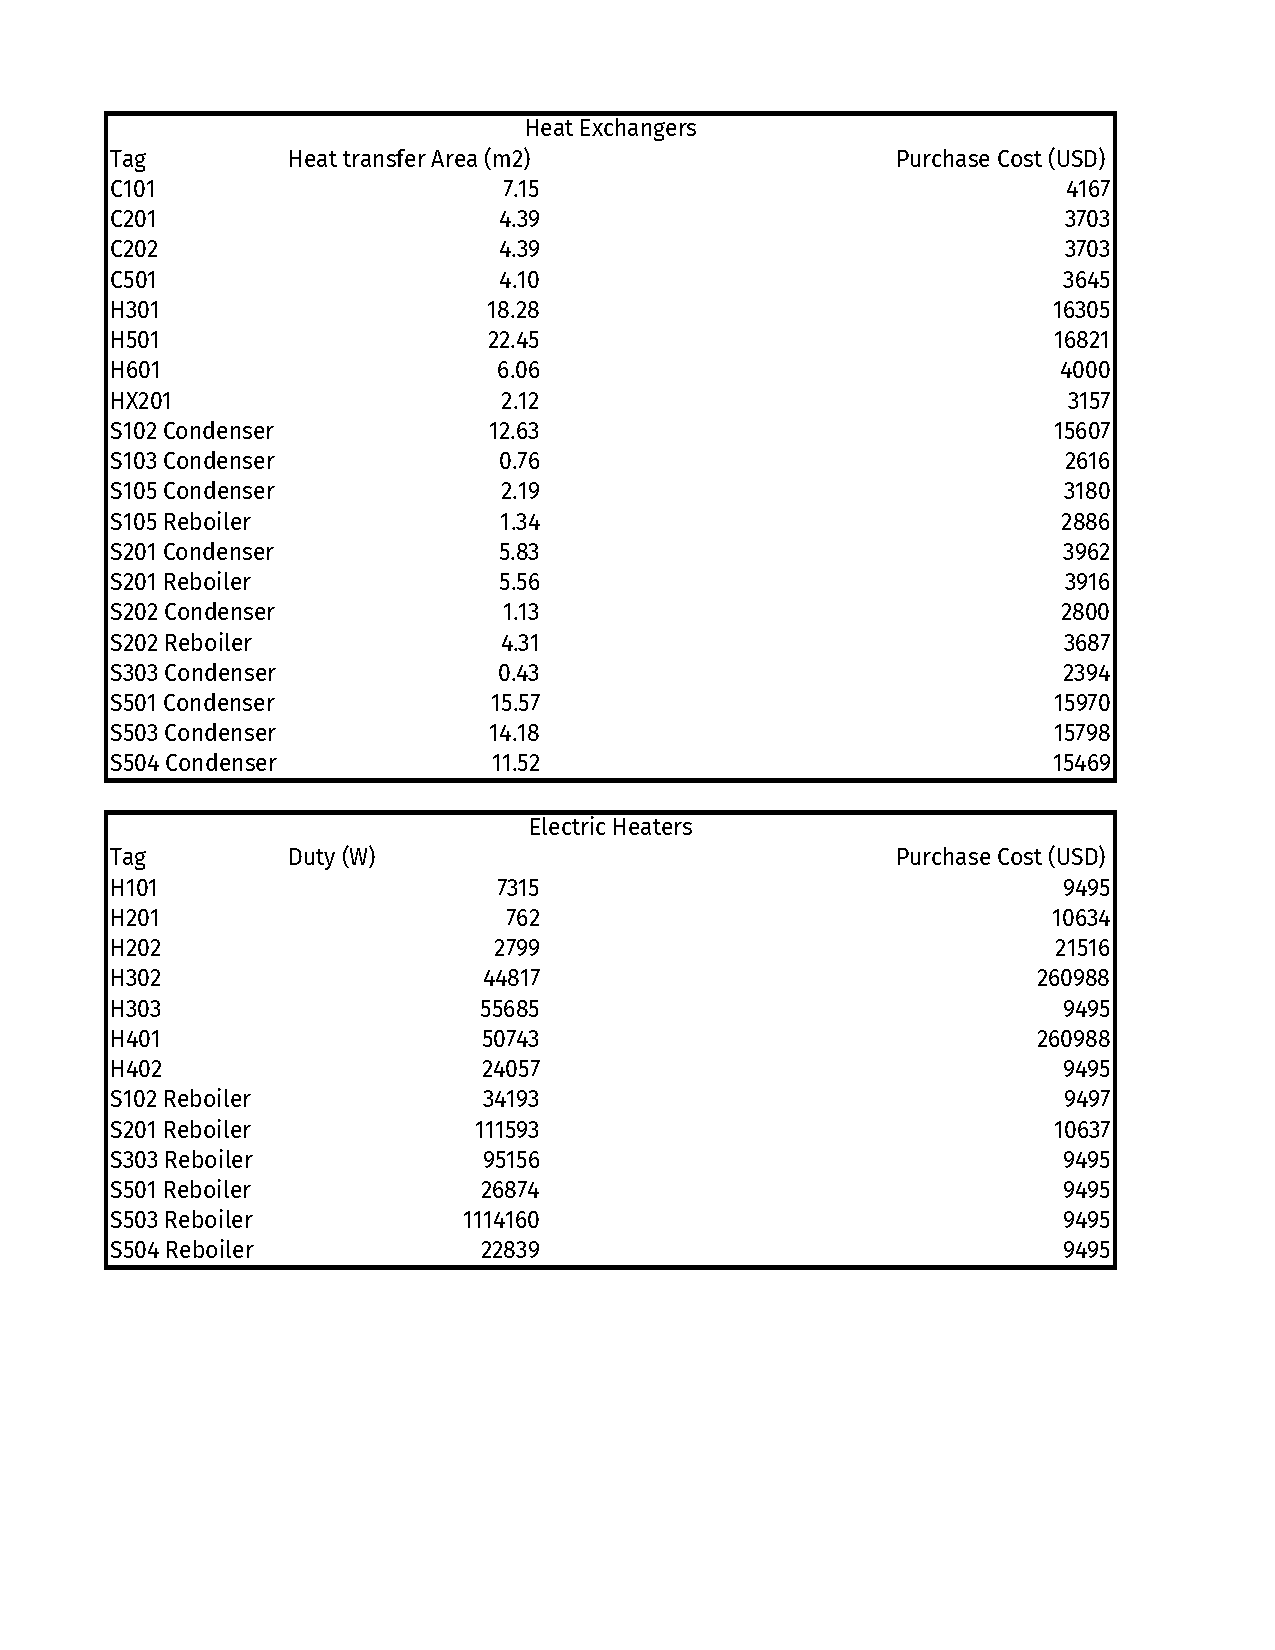
\includepdf[pages=-]{figures/Equipment List.pdf}